\documentclass[10pt,twopage]{acmsiggraph}

\usepackage{fancyheadings} % we need page numbers...
\usepackage{times}
\usepackage{graphicx}
\usepackage{hyperref}

% allow for many figures and tables on one page
\renewcommand{\topfraction}{1.0} % all floats ok
\setcounter{totalnumber}{10}     % #floats = 10
\renewcommand{\textfraction}{0.0} % no text ok
\renewcommand{\dbltopfraction}{0.4}


% override page numbering conventions of the acm style
\pagestyle{fancyplain}
\lhead[\name]{}		% author name on the left for even pages
\rhead[]{\name}		% and on the right for odd pages
\setcounter{page}{1}	% I need to change this line for the proceedings
 


%%%%%%%%%%%
%
% Do not change anything above this line!!!
%
%%%%%%%%%%%




\begin{document}

%%%%%%%%%%%%%%%%%%%%%%%%%%%%%%%%%%%%%%%%%%%%%%%%%%%%%%%%%%%%%%%%%%%%%%%%%%%%%%%
%%%%%%%%%%%%%%%%%%%%%%%%%%%%%%%%%%%%%%%%%%%%%%%%%%%%%%%%%%%%%%%%%%%%%%%%%%%%%%%
%
% Title and author(s)
%
%%%%%%%%%%%%%%%%%%%%%%%%%%%%%%%%%%%%%%%%%%%%%%%%%%%%%%%%%%%%%%%%%%%%%%%%%%%%%%%
%%%%%%%%%%%%%%%%%%%%%%%%%%%%%%%%%%%%%%%%%%%%%%%%%%%%%%%%%%%%%%%%%%%%%%%%%%%%%%%

\title{Term Project for CPSC514 -- Irradiance Cache Splatting}

\newcommand\name{Ben Jones}

\author{\name\\
\\
Department of Computer Science\\
The University of British Columbia}

\maketitle

%%%%%%%%%%%%%%%%%%%%%%%%%%%%%%%%%%%%%%%%%%%%%%%%%%%%%%%%%%%%%%%%%%%%%%%%%%%%%%%
%%%%%%%%%%%%%%%%%%%%%%%%%%%%%%%%%%%%%%%%%%%%%%%%%%%%%%%%%%%%%%%%%%%%%%%%%%%%%%%
%
% Abstract
%
%%%%%%%%%%%%%%%%%%%%%%%%%%%%%%%%%%%%%%%%%%%%%%%%%%%%%%%%%%%%%%%%%%%%%%%%%%%%%%%
%%%%%%%%%%%%%%%%%%%%%%%%%%%%%%%%%%%%%%%%%%%%%%%%%%%%%%%%%%%%%%%%%%%%%%%%%%%%%%%

\begin{abstract}
  This document describes the procedure for projects in CPSC 514. The
  document also serves as an example for simple \LaTeX\ documents.
\end{abstract}

%%%%%%%%%%%%%%%%%%%%%%%%%%%%%%%%%%%%%%%%%%%%%%%%%%%%%%%%%%%%%%%%%%%%%%%%%%%%%%%
%%%%%%%%%%%%%%%%%%%%%%%%%%%%%%%%%%%%%%%%%%%%%%%%%%%%%%%%%%%%%%%%%%%%%%%%%%%%%%%
%
% Introduction
%
%%%%%%%%%%%%%%%%%%%%%%%%%%%%%%%%%%%%%%%%%%%%%%%%%%%%%%%%%%%%%%%%%%%%%%%%%%%%%%%
%%%%%%%%%%%%%%%%%%%%%%%%%%%%%%%%%%%%%%%%%%%%%%%%%%%%%%%%%%%%%%%%%%%%%%%%%%%%%%%

\section{Introduction}
\label{Intro}

Fast, realistic rendering of complex scenes is one of the major goals of computer graphics.  Methods based on Monte-Carlo ray tracing provide photorealistic results but are far too slow to be used in interactive applications \cite{cook1984distributed}.  One of the problems associated with these techniques is that they rely on complex data structures, meaning that they cannot easily take advantage of today's extremely powerful GPUs.  The algorithm presented in \cite{mainpaper} seeks to approximate the global illumination solution using operations that are well suited to running on a GPU.  For my course project, I implemented part of their "irradiance cache splatting" algorithm for diffuse scenes.

The key observations this algorithm exploits are first: in typical scenes, most lighting in the scene comes from the direct component, and the first bounce of light off of other surfaces.  Second, the indirect light contribution tends to change slowly across surfaces.  

The algorithm adapts a technique from \cite{ward1988ray} which samples the indirect lighting at points interpolates between them to generate an approximation of total indirect contribution.  This result is combined with the direct illumination component to create the final image.  In the original algorithm, the interpolation is performed via nearest-neighbor queries, which is not an acceptable approach when using a GPU.  In the improved algorithm from \cite{mainpaper}, both the sampling and interpolation leverage the GPU's parallel processing ability.  The sampled values are computed by rendering the environment from points in the scene and performing a weighted summation of the pixel values.  The interpolation is performed by treating each sample as a sphere with radius proportional to its estimated error and "splatting" all the spheres onto a buffer.  The samples can be processed separately and no information about neighbors is required.

The rest of the paper describes the algorithm in more detail, my implementation, and my results.

\section{Algorithm}
The algorithm consists of 5 main steps.  
\begin{enumerate}
\item Irradiance records are computed for points in the scene, chosen at random in my implementation.  
\item The records are splatted into a buffer recording the indirect lighting contribution.  
\item The buffer is examined, and new samples are generated and splatted.  
\item The direct illumination component is computed.  
\item The indirect and direct contributions are combined to generate the final image.  
\end{enumerate}

Step 1 and 3 are computed using both the GPU and CPU.  Steps 2, 4 and 5 are performed using only the GPU.

\subsection{Record Computation}
Each record is generated by rendering the scene at a point visible from the viewpoint, in the direction of its normal.  The scene is rendered from the eye, and the positions, normals, and surface properties of all visible points in the scene is stored on the CPU so viewing transform can be set up quickly.  The rendering is performed using shadow mapping so the first-bounce visible light measured at each sample is accurate.  The image is then copied to the CPU where a summation is performed as in \cite{larsen2004simulating}: 
$$
E = \sum_{x,y}\frac{p(x,y)\Delta A_f}{\pi(x^2 + y^2 +1)^2}
$$
where E is the computed irradiance, $p(x,y)$ is the pixel value at $(x,y)$,  and $\Delta A_f$ is the area of each pixel.  While this calculation can be performed on the GPU using mipmap generation, \cite{mainpaper} performed it on the CPU, so my implementation does as well.  The irradiance for each color channel (r,g,b) is computed separately.

Another aggregate quantity, the harmonic mean distance to objects, is computed at each sample by summation of the depth values of visible objects.  This computation is also performed on the CPU.

Ideally, the entire hemisphere around the record point would be sampled, but sampling a plane is much easier and faster to do using the GPU's rasterization engine.  In order to minimize error, a very wide field of view angle, and very short front clipping plane distance are used.    

\subsection{Record Splatting}
Each sample as computed in step 1 is projected onto the image plane as a sphere, representing which visible pixels have similar indirect contribution.  The spheres have radius = $aR_k$ where $a$ is a tunable parameter, and $R_k$ is the harmonic mean distance to objects visible at sample $k$.

For each pixel in the buffer in the bounding box of the sphere associated with record $k$, a weight, $w$ is computed as
$$
w_k = \frac{1}{\frac{p - p_k}{R_k} + \sqrt{1 - n \cdot n_k}}
$$
where p is the position of the point, $p_k$ is the position of the associated sample, $n$ and $n_k$ are the normals of the point and associated sample, respectively.  The weight is computed that nearby points with similar normals are given high weight, since they are more likely to have similar indirect contributions.

For each pixel in the bounding box, if this value is greater than the $1/a$ tolerance, the associated irradiance is added to the buffer: 
\begin{eqnarray*}
buf(x,y).L_0 &+=& wL_0,  \\
buf.w &+=& w
\end{eqnarray*}
where $L_0$ is the estimated irradiance at $(x,y)$.  \cite{mainpaper} computes $L_0$ taking the gradiants of the sample into account, but in my implementation, $L_0 = E_k*\rho_d$, the sampled irradiance value multiplied by the diffuse reflectance of the surface.  

\subsection{Buffer Examination}
The splatting for all samples is performed simultaneously on the GPU, however, especially for the first frame, the scene many not be sampled adequately.  To remedy this, the splat buffer is read onto the CPU, and each pixel is examined.  If its weight is less than $a$, a new sample is generated at that point.  Still on the CPU, the weight is splatted onto the CPU copy of the buffer so that nearby pixels have their weights updated, and fewer samples will be generated.  After traversing the buffer, the newly generated samples are splatted onto the GPU copy of the buffer.

\subsection{Direct Illumination}
The direction illumination component is computed by rendering the scene from the viewpoint with shadow mapping.  Antialiasing is performed to prevent jagged edges on shadow boundaries.

\subsection{Combining Direct and Indirect Components}
In my implementation, the direct and indirect contributions were combined with a simple weighted sum.  This turned out not to be an adequate approach, and the weighting results in a tradeoff between the subtle details of color bleeding and washing out the shading of the rest of the scene.

\section{Implementation}
My implementation was written in c++ using OpenGL and GLSL to control GPU execution.  It makes heavy use of Frame Buffer Objects (FBO) for rendering to textures.  In most cases these textures can remain on the GPU, so there is little overhead in reading from them at a future step.  Floating point textures are used to store values like positions (or depth) so that their values are not clamped onto the range [0, 1].

%\subsection{Scene Input}

\subsection{Retrieving Visible Object and Normal Data}
For the CPU based steps, and for passing data to the GPU, a record of the visible points in the scene along with their normal vectors and material properties must be stored on the CPU.  This is accomplished by rendering the scene to a floating point texture which is read back to the CPU.  

\subsection{Shadow Mapped Rendering}
Both the direct illumination step, and record computations steps rely on generating an accurately shadowed view of the scene.  My implementation uses the shadow mapping algorithm described in \cite{orangebook}.  The scene is first rendered with front face culling from the viewpoint of each light in the scene.  Each one of these views is stored in layer of a depth texture array.  The scene is then rendered from the viewpoint with backface culling.  A vertex shader computes the coordinates of each vertex in the eye-coordinates for each light.  Finally a fragment compares the distance from each fragment to the light source to the associated depth texture, lighting points that have smaller depth than the texture.  

Due to numerical errors, surfaces can exhibit a moire pattern, which is prevented by adding a small tolerance to the depth value of each fragment.  Also, when projected, aliasing artifacts of the shadow maps can be quite noticeable.  To prevent jagged shadow edges, 4 dithered samples are examined for each light for each fragment.

\subsection{Record Computation}
When a new record is requested, the scene is rendered, shadow mapped, from that point in the direction of its normal vector, to a texture.  Since many of these records are created, they are rendered at low resolution to save time in transferring to and summing them on the CPU.    The texture is copied from the GPU to the CPU.  The depth and pixel values are summed to compute the record's harmonic mean distance and irradiance values.  

\cite{mainpaper} and \cite{larsen2004simulating} note that this summation can be performed using mipmap generation on the GPU, but \cite{mainpaper} claimed the CPU based approach performed better.

\subsection{Splatting}
The splatting process must be performed on both the GPU and CPU during different parts of the algorithm.  The CPU implementation is necessary so that when a new sample is computed in an under sampled section of the image, the sample can impact its neighboring values.  If just the GPU implementation was used, after each new record was created and splatted, the splat buffer would have to be read back to the CPU again before the traversal could proceed.  Therefore, the CPU based implementation prevents significant time from being used transferring the buffer back and forth between the GPU and CPU.

\subsubsection{GPU Implementation}
In the GPU implementation, the spheres are rendered as quads that bound the actual spheres.  The coordinates of the vertices of the quad are computed using a vertex shader.  The center of the sphere is passed in as all 4 vertices of the quad, and the fragment shader computes the vertical and horizontal vectors that are normal to the eye vector, in eye-space, as shown in fig \ref{boundingBox}.  This results in a slight overestimation of the sphere, but inclusion can be checked exactly in the fragment shader, resulting in only a small amount of wasted computation.  

\begin{figure}[htbp]
\begin{center}
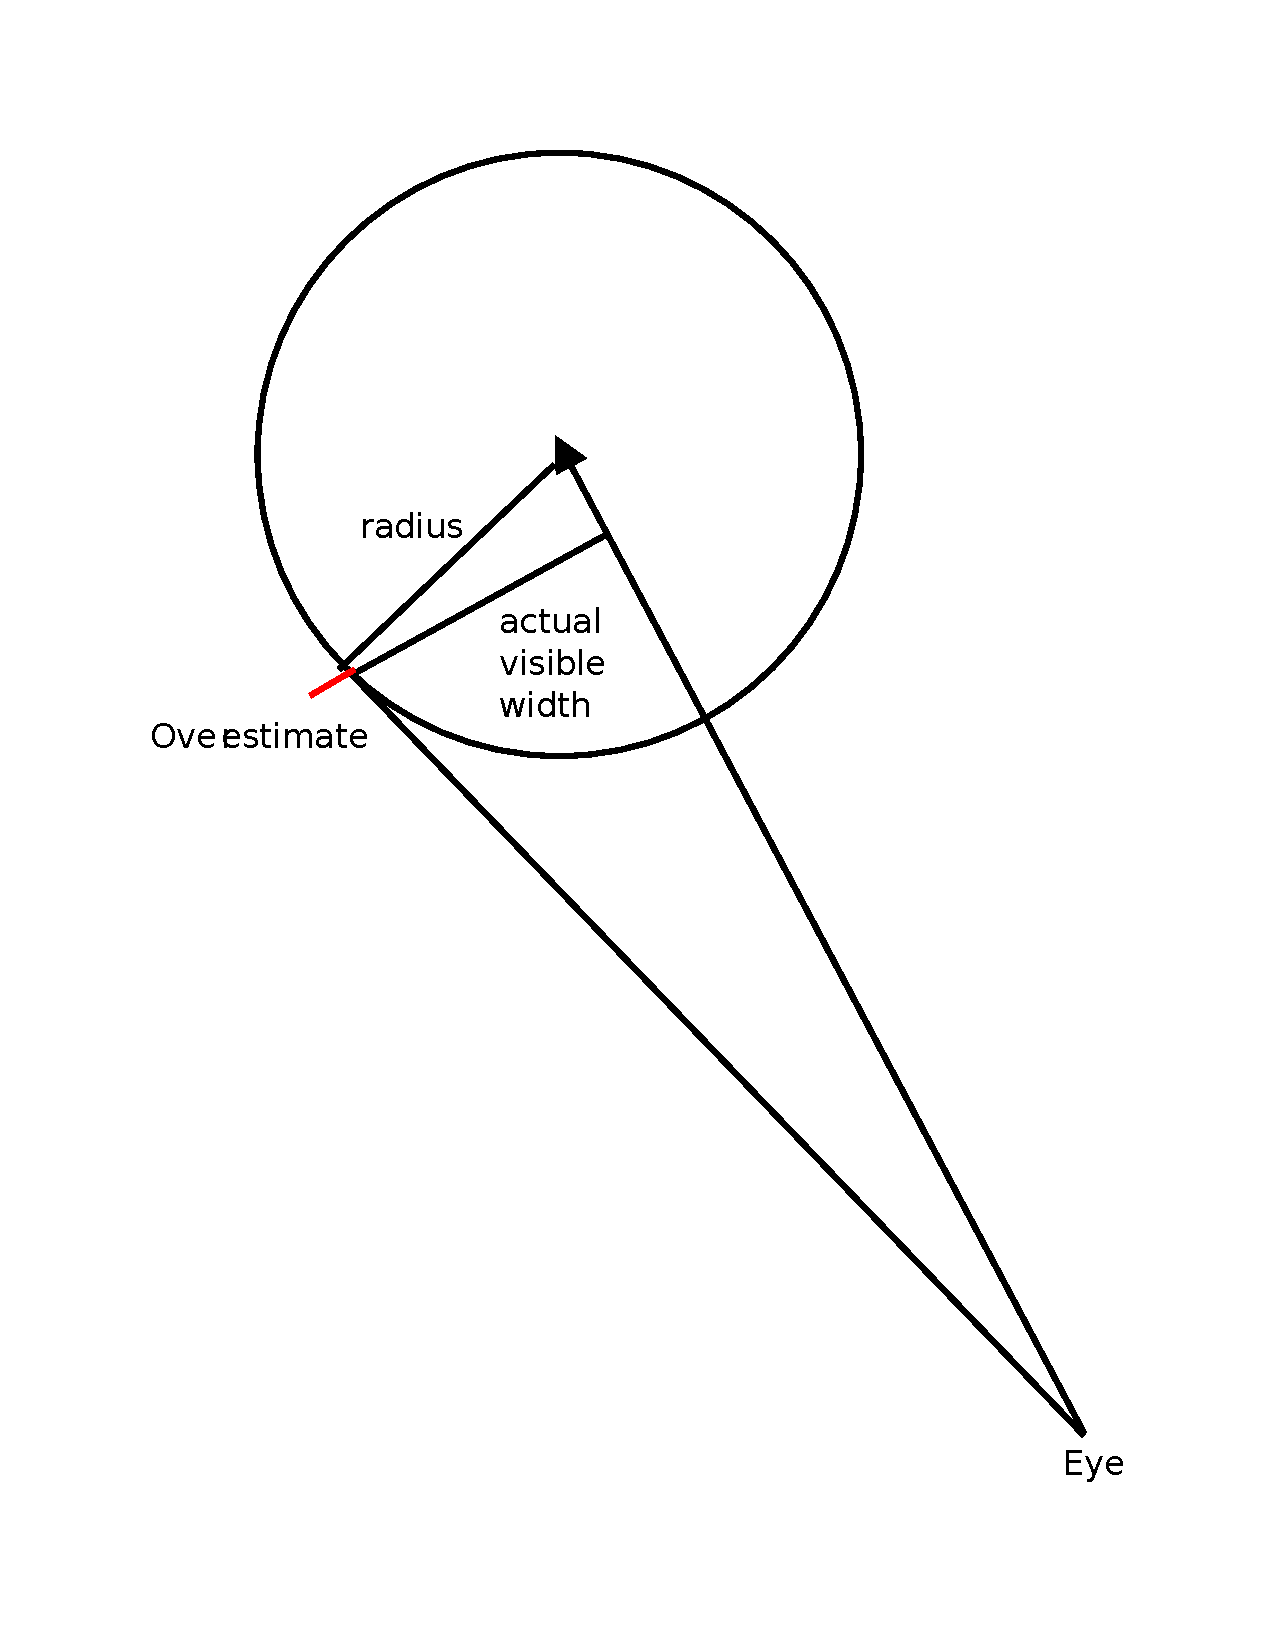
\includegraphics[scale = .5]{splatEye.pdf}
\caption{Computation of sphere bounding box in vertex shader}
\label{boundingBox}
\end{center}
\end{figure}

The splatting process is performed with blending enabled, so that all contributions are summed together.  The contributions are computed in the fragment shader as described in section 2.2.  The $p$, $n$ and $\rho_d$ values are retrieved via texture lookup on the textures created in section 3.1 

\subsubsection{CPU Implementation}
The same algorithm from the previous section is performed on the CPU.  Since the rasterization engine is not available, the bounding box is computed by finding the range of x and y pixel values that are projected onto image plane.  Since color information is not needed in this step, only weight information is recorded to the CPU copy of the buffer.

After all the new records have been created, they are given to the GPU and splatted using the GPU implementation.

\subsection{Combining Direct and Indirect Results}
The results are combined with a fragment shader.  A full-screen quad is rendered with the direct and indirect contributions retrieved by texture lookup.  The colors of the indirect buffer are normalized by dividing the r,g,b values by the associated $w$ value.

\section{Results}
All images were rendered at 800x800 resolution on a quad-core workstation with GeForce 8800GT GPU with 512MB graphics memory.  My implementation was tested on a Cornell Box type scene with pure red and green walls, a white wall, ceiling and floor.  There are 2 white cubes and 3 light sources, one at the center of the ceiling, and two outside the box.  Fig \ref{direct} shows the direct lighting contribution.

\begin{figure}[htbp]
\begin{center}
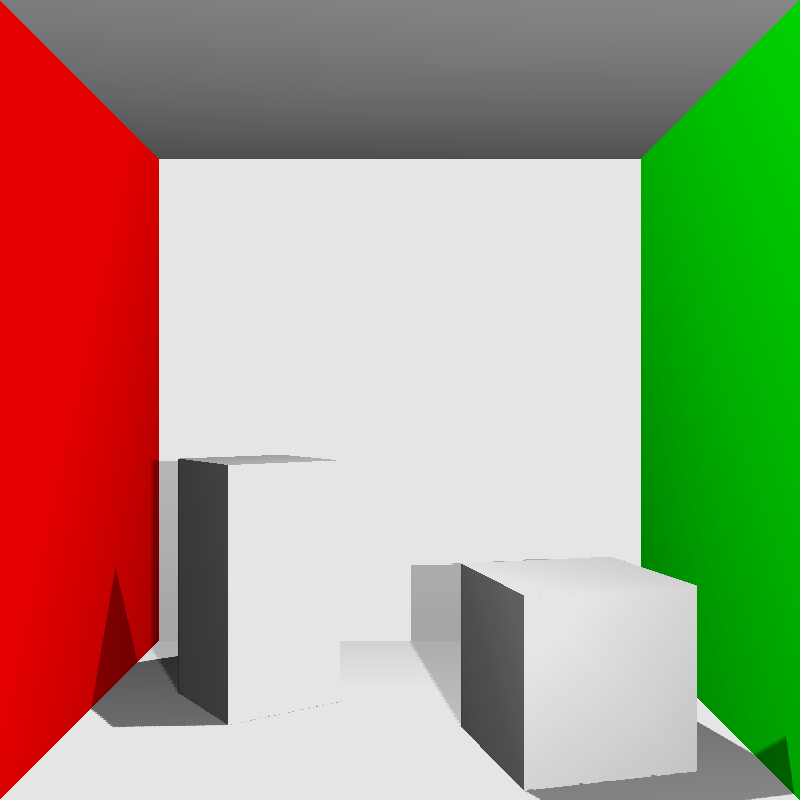
\includegraphics[scale = .3]{directIllumination.png}
\caption{Direct illumination result of Cornell Box scene.}
\label{direct}
\end{center}
\end{figure}

The indirect lighting is computed in 3 steps.  First, the 1000 samples at random points in the scene are generated and splatted, shown in fig \ref{splat1000}.  Then, the CPU traversal produces more samples, which are then splatted (fig\ref{splatAll}) and normalized (fig\ref{splatNorm}).

\begin{figure}[htbp]
\begin{center}
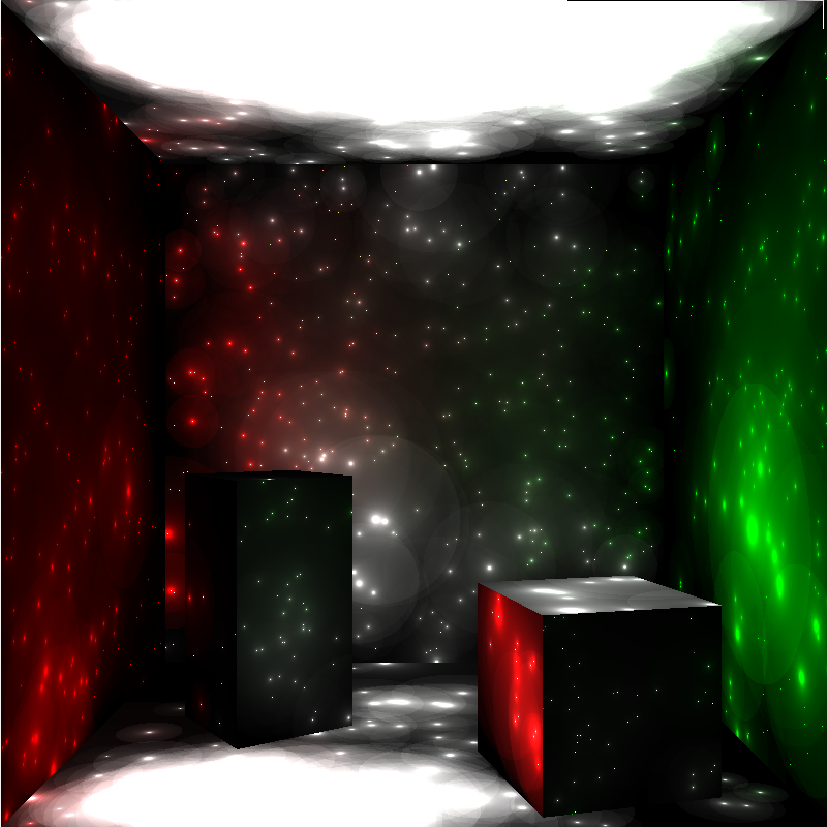
\includegraphics[scale = .3]{1000Samples.png}
\caption{The first 1000 samples s result of Cornell Box scene.}
\label{splat1000}
\end{center}
\end{figure}

\begin{figure}[htbp]
\begin{center}
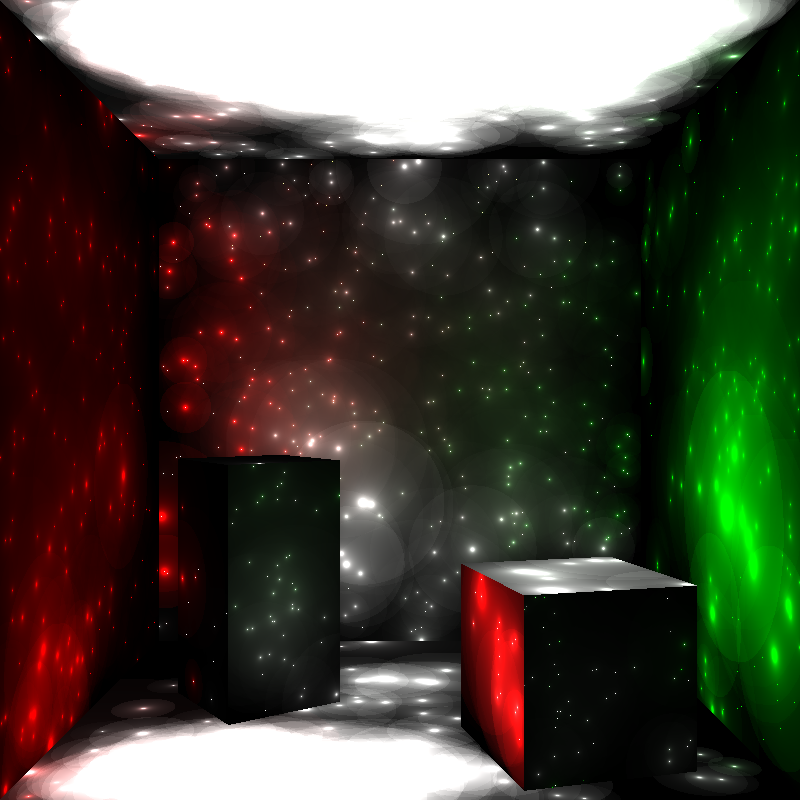
\includegraphics[scale = .3]{firstBounceLight.png}
\caption{Splat buffer after CPU traversal.}
\label{splatAll}
\end{center}
\end{figure}

\begin{figure}[htbp]
\begin{center}
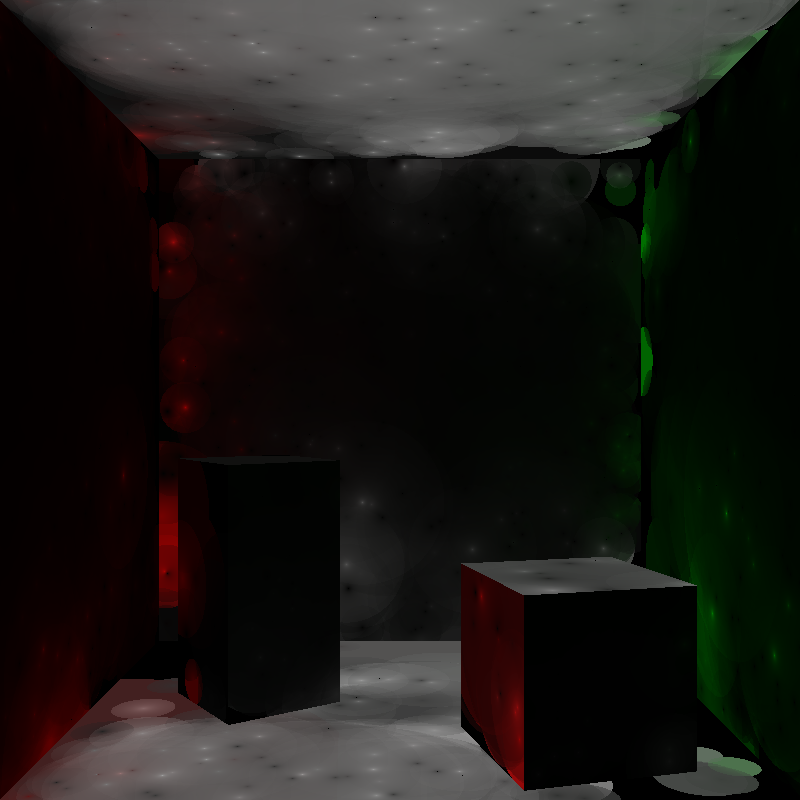
\includegraphics[scale = .3]{indirectContribution.png}
\caption{Splat buffer after normalization.}
\label{splatNorm}
\end{center}
\end{figure}

Finally the direct and indirect contributions are combined to generate the final image, fig \ref{final}.

\begin{figure}[htbp]
\begin{center}
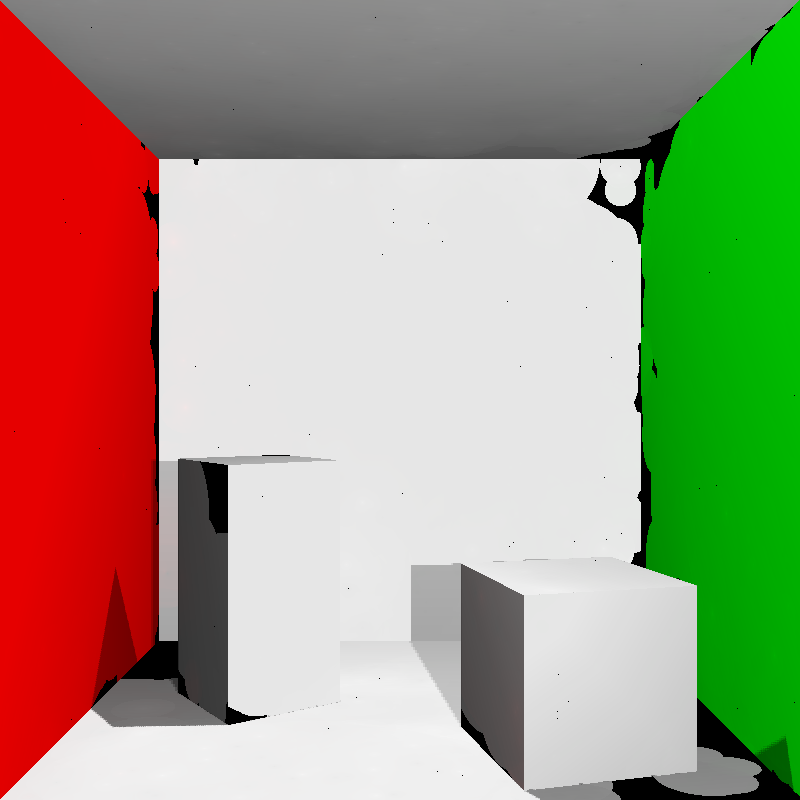
\includegraphics[scale = .3]{finalResult.png}
\caption{Final combined image}
\label{final}
\end{center}
\end{figure}

Generating the first 1000 samples took 1.11 seconds.  The direct illumination rendering took 0.00195 seconds.  511 new records were generated.  It took .0195 seconds to splat the original records, 1.04 seconds to perform the CPU traversal, and .00107 seconds to splat the 511 newly created records.  The final pass combining the two images took .00203 seconds.  Record generation and traversing the splat buffer in the CPU took, by far, the most time.  If the viewpoint were moved after a sufficient number of samples had been generated, subsequent frames would likely be very fast to generate, but I didn't have time to test this.

The results show that color bleeding is correctly accounted for, especially in the shadowed regions of the boxes and the floor near the red and green walls.  The final image, however is flawed.  There are several reasons for this.  The biggest problem is that the naive blending of the direct and indirect images saturates parts of the image, like the walls, while under-representing the color bleeding in the floors and shadowed regions.  A better blending scheme would result in a much better image.

Second, the indirect lighting has lots of visual artifacts, especially perfectly circular shapes.  These could be improved by either accounting for the sample gradients as described in \cite{mainpaper} or by performing smoothing operation on the indirect contribution image.  

\section{Conclusion}
I implemented part of the irradiance cache splatting algorithm described in \cite{mainpaper} for diffuse surfaces.  While the indirect contribution on its own was visually plausible, the combination with direct lighting was not successful, resulting in a low quality final output.  The system does not run at true interactive rates, but is still reasonably fast, at least on simple scenes.  With an improved blending algorithm and using the sample gradient information, the system I developed could be used to generate fast, high quality renderings of diffuse scenes.


\bibliographystyle{acmsiggraph}
{\small\bibliography{project.bib}}

%%%%%%%%%%%
%
% Do not change anything below this line!!!
%
%%%%%%%%%%%


% adds an empty page to documents with odd page number. This is to
% make sure that the first page of every paper starts at an odd page.
\cleardoublepage

\end{document}

% LocalWords:  CPSC Heidrich PDF cpsc tex dvi xdvi BibTeX bibtex PostScript ps
% LocalWords:  dvips Ppdf pdf pdflatex EPS PNG includegraphics
